\documentclass{ximera}

%\usepackage{todonotes}

\newcommand{\todo}{}

\usepackage{esint} % for \oiint
\ifxake%%https://math.meta.stackexchange.com/questions/9973/how-do-you-render-a-closed-surface-double-integral
\renewcommand{\oiint}{{\large\bigcirc}\kern-1.56em\iint}
\fi


\graphicspath{
  {./}
  {ximeraTutorial/}
  {basicPhilosophy/}
  {functionsOfSeveralVariables/}
  {normalVectors/}
  {lagrangeMultipliers/}
  {vectorFields/}
  {greensTheorem/}
  {shapeOfThingsToCome/}
  {dotProducts/}
  {partialDerivativesAndTheGradientVector/}
  {../productAndQuotientRules/exercises/}
  {../normalVectors/exercisesParametricPlots/}
  {../continuityOfFunctionsOfSeveralVariables/exercises/}
  {../partialDerivativesAndTheGradientVector/exercises/}
  {../directionalDerivativeAndChainRule/exercises/}
  {../commonCoordinates/exercisesCylindricalCoordinates/}
  {../commonCoordinates/exercisesSphericalCoordinates/}
  {../greensTheorem/exercisesCurlAndLineIntegrals/}
  {../greensTheorem/exercisesDivergenceAndLineIntegrals/}
  {../shapeOfThingsToCome/exercisesDivergenceTheorem/}
  {../greensTheorem/}
  {../shapeOfThingsToCome/}
  {../separableDifferentialEquations/exercises/}
  {vectorFields/}
}

\newcommand{\mooculus}{\textsf{\textbf{MOOC}\textnormal{\textsf{ULUS}}}}

\usepackage{tkz-euclide}
\usepackage{tikz}
\usepackage{tikz-cd}
\usetikzlibrary{arrows}
\tikzset{>=stealth,commutative diagrams/.cd,
  arrow style=tikz,diagrams={>=stealth}} %% cool arrow head
\tikzset{shorten <>/.style={ shorten >=#1, shorten <=#1 } } %% allows shorter vectors

\usetikzlibrary{backgrounds} %% for boxes around graphs
\usetikzlibrary{shapes,positioning}  %% Clouds and stars
\usetikzlibrary{matrix} %% for matrix
\usepgfplotslibrary{polar} %% for polar plots
\usepgfplotslibrary{fillbetween} %% to shade area between curves in TikZ
%\usetkzobj{all}
\usepackage[makeroom]{cancel} %% for strike outs
%\usepackage{mathtools} %% for pretty underbrace % Breaks Ximera
%\usepackage{multicol}
\usepackage{pgffor} %% required for integral for loops



%% http://tex.stackexchange.com/questions/66490/drawing-a-tikz-arc-specifying-the-center
%% Draws beach ball
\tikzset{pics/carc/.style args={#1:#2:#3}{code={\draw[pic actions] (#1:#3) arc(#1:#2:#3);}}}



\usepackage{array}
\setlength{\extrarowheight}{+.1cm}
\newdimen\digitwidth
\settowidth\digitwidth{9}
\def\divrule#1#2{
\noalign{\moveright#1\digitwidth
\vbox{\hrule width#2\digitwidth}}}




% \newcommand{\RR}{\mathbb R}
% \newcommand{\R}{\mathbb R}
% \newcommand{\N}{\mathbb N}
% \newcommand{\Z}{\mathbb Z}

\newcommand{\sagemath}{\textsf{SageMath}}


%\renewcommand{\d}{\,d\!}
%\renewcommand{\d}{\mathop{}\!d}
%\newcommand{\dd}[2][]{\frac{\d #1}{\d #2}}
%\newcommand{\pp}[2][]{\frac{\partial #1}{\partial #2}}
% \renewcommand{\l}{\ell}
%\newcommand{\ddx}{\frac{d}{\d x}}

% \newcommand{\zeroOverZero}{\ensuremath{\boldsymbol{\tfrac{0}{0}}}}
%\newcommand{\inftyOverInfty}{\ensuremath{\boldsymbol{\tfrac{\infty}{\infty}}}}
%\newcommand{\zeroOverInfty}{\ensuremath{\boldsymbol{\tfrac{0}{\infty}}}}
%\newcommand{\zeroTimesInfty}{\ensuremath{\small\boldsymbol{0\cdot \infty}}}
%\newcommand{\inftyMinusInfty}{\ensuremath{\small\boldsymbol{\infty - \infty}}}
%\newcommand{\oneToInfty}{\ensuremath{\boldsymbol{1^\infty}}}
%\newcommand{\zeroToZero}{\ensuremath{\boldsymbol{0^0}}}
%\newcommand{\inftyToZero}{\ensuremath{\boldsymbol{\infty^0}}}



% \newcommand{\numOverZero}{\ensuremath{\boldsymbol{\tfrac{\#}{0}}}}
% \newcommand{\dfn}{\textbf}
% \newcommand{\unit}{\,\mathrm}
% \newcommand{\unit}{\mathop{}\!\mathrm}
% \newcommand{\eval}[1]{\bigg[ #1 \bigg]}
% \newcommand{\seq}[1]{\left( #1 \right)}
% \renewcommand{\epsilon}{\varepsilon}
% \renewcommand{\phi}{\varphi}


% \renewcommand{\iff}{\Leftrightarrow}

% \DeclareMathOperator{\arccot}{arccot}
% \DeclareMathOperator{\arcsec}{arcsec}
% \DeclareMathOperator{\arccsc}{arccsc}
% \DeclareMathOperator{\si}{Si}
% \DeclareMathOperator{\scal}{scal}
% \DeclareMathOperator{\sign}{sign}


%% \newcommand{\tightoverset}[2]{% for arrow vec
%%   \mathop{#2}\limits^{\vbox to -.5ex{\kern-0.75ex\hbox{$#1$}\vss}}}
% \newcommand{\arrowvec}[1]{{\overset{\rightharpoonup}{#1}}}
% \renewcommand{\vec}[1]{\arrowvec{\mathbf{#1}}}
% \renewcommand{\vec}[1]{{\overset{\boldsymbol{\rightharpoonup}}{\mathbf{#1}}}}

% \newcommand{\point}[1]{\left(#1\right)} %this allows \vector{ to be changed to \vector{ with a quick find and replace
% \newcommand{\pt}[1]{\mathbf{#1}} %this allows \vec{ to be changed to \vec{ with a quick find and replace
% \newcommand{\Lim}[2]{\lim_{\point{#1} \to \point{#2}}} %Bart, I changed this to point since I want to use it.  It runs through both of the exercise and exerciseE files in limits section, which is why it was in each document to start with.

% \DeclareMathOperator{\proj}{\mathbf{proj}}
% \newcommand{\veci}{{\boldsymbol{\hat{\imath}}}}
% \newcommand{\vecj}{{\boldsymbol{\hat{\jmath}}}}
% \newcommand{\veck}{{\boldsymbol{\hat{k}}}}
% \newcommand{\vecl}{\vec{\boldsymbol{\l}}}
% \newcommand{\uvec}[1]{\mathbf{\hat{#1}}}
% \newcommand{\utan}{\mathbf{\hat{t}}}
% \newcommand{\unormal}{\mathbf{\hat{n}}}
% \newcommand{\ubinormal}{\mathbf{\hat{b}}}

% \newcommand{\dotp}{\bullet}
% \newcommand{\cross}{\boldsymbol\times}
% \newcommand{\grad}{\boldsymbol\nabla}
% \newcommand{\divergence}{\grad\dotp}
% \newcommand{\curl}{\grad\cross}
%\DeclareMathOperator{\divergence}{divergence}
%\DeclareMathOperator{\curl}[1]{\grad\cross #1}
% \newcommand{\lto}{\mathop{\longrightarrow\,}\limits}

% \renewcommand{\bar}{\overline}

\colorlet{textColor}{black}
\colorlet{background}{white}
\colorlet{penColor}{blue!50!black} % Color of a curve in a plot
\colorlet{penColor2}{red!50!black}% Color of a curve in a plot
\colorlet{penColor3}{red!50!blue} % Color of a curve in a plot
\colorlet{penColor4}{green!50!black} % Color of a curve in a plot
\colorlet{penColor5}{orange!80!black} % Color of a curve in a plot
\colorlet{penColor6}{yellow!70!black} % Color of a curve in a plot
\colorlet{fill1}{penColor!20} % Color of fill in a plot
\colorlet{fill2}{penColor2!20} % Color of fill in a plot
\colorlet{fillp}{fill1} % Color of positive area
\colorlet{filln}{penColor2!20} % Color of negative area
\colorlet{fill3}{penColor3!20} % Fill
\colorlet{fill4}{penColor4!20} % Fill
\colorlet{fill5}{penColor5!20} % Fill
\colorlet{gridColor}{gray!50} % Color of grid in a plot

\newcommand{\surfaceColor}{violet}
\newcommand{\surfaceColorTwo}{redyellow}
\newcommand{\sliceColor}{greenyellow}




\pgfmathdeclarefunction{gauss}{2}{% gives gaussian
  \pgfmathparse{1/(#2*sqrt(2*pi))*exp(-((x-#1)^2)/(2*#2^2))}%
}


%%%%%%%%%%%%%
%% Vectors
%%%%%%%%%%%%%

%% Simple horiz vectors
\renewcommand{\vector}[1]{\left\langle #1\right\rangle}


%% %% Complex Horiz Vectors with angle brackets
%% \makeatletter
%% \renewcommand{\vector}[2][ , ]{\left\langle%
%%   \def\nextitem{\def\nextitem{#1}}%
%%   \@for \el:=#2\do{\nextitem\el}\right\rangle%
%% }
%% \makeatother

%% %% Vertical Vectors
%% \def\vector#1{\begin{bmatrix}\vecListA#1,,\end{bmatrix}}
%% \def\vecListA#1,{\if,#1,\else #1\cr \expandafter \vecListA \fi}

%%%%%%%%%%%%%
%% End of vectors
%%%%%%%%%%%%%

%\newcommand{\fullwidth}{}
%\newcommand{\normalwidth}{}



%% makes a snazzy t-chart for evaluating functions
%\newenvironment{tchart}{\rowcolors{2}{}{background!90!textColor}\array}{\endarray}

%%This is to help with formatting on future title pages.
\newenvironment{sectionOutcomes}{}{}



%% Flowchart stuff
%\tikzstyle{startstop} = [rectangle, rounded corners, minimum width=3cm, minimum height=1cm,text centered, draw=black]
%\tikzstyle{question} = [rectangle, minimum width=3cm, minimum height=1cm, text centered, draw=black]
%\tikzstyle{decision} = [trapezium, trapezium left angle=70, trapezium right angle=110, minimum width=3cm, minimum height=1cm, text centered, draw=black]
%\tikzstyle{question} = [rectangle, rounded corners, minimum width=3cm, minimum height=1cm,text centered, draw=black]
%\tikzstyle{process} = [rectangle, minimum width=3cm, minimum height=1cm, text centered, draw=black]
%\tikzstyle{decision} = [trapezium, trapezium left angle=70, trapezium right angle=110, minimum width=3cm, minimum height=1cm, text centered, draw=black]

\author{Jim Talamo (edited)}

\title{What is a series}

 
 
 
\begin{document}
\begin{abstract}
adding a sequence
\end{abstract}
\maketitle

In the previous sections, we've seen several examples of sequences.  If we have a sequence $\{a_n\}_{n=1}$, then we can ask two important questions about it.

\begin{itemize}
\item \textbf{\textcolor{purple!85!blue}{Do the numbers in the list approach a finite value?}} 
\item \textbf{\textcolor{purple!85!blue}{If so, what is the value?}} 
\end{itemize}


The first question is called an \textbf{\textcolor{purple!85!blue}{existence}} question.  Does the limit exist?  This is a yes or no question.

If the answer is yes (the limit exists), then we come to the second question. \\


In this section, we propose a different view of a sequence of numbers.  We can view them as terms in a partial summation, where we keep adding on more terms, like digits in a decimal expansion.







\begin{example}


Consider the sequence $(a_n)_{n=1} = 5, 8, 7, 9, 10, 10, 13, \cdots$. \\

This sequence could be viewed as


\begin{align*}
a_1 & = 5  & = 5 \\
a_2 & = 8  & = 5 + 3 \\
a_3 & = 7  & = 5 + 3 - 1 \\
a_4 & = 9  & = 5 + 3 - 1 + 2 \\
a_5 & = 10 & = 5 + 3 - 1 + 2 + 1 \\
a_6 & = 10 & = 5 + 3 - 1 + 2 + 1 + 0 \\
a_7 & = 13 & = 5 + 3 - 1 + 2 + 1 + 0 + 3
\end{align*}


The terms of the original sequence, $(a_n)$, are each the sum of the first $n$ numbers from the sequence 

\[
(b_k)_{k=1} = 5, 3, -1, 2, 1, 0, 3, \cdots
\]





\end{example}


We could go the other way as well.  We could begin with a sequence and then create another sequence where the terms are the partial sums of the original sequence.








\begin{example}


Consider the sequence $(a_k)_{k=1} = 3, 6, 2, 1, 0, 4, \cdots$. \\

Define a new sequence $(s_n)_{n=1}$ as 


\[
(s_n)_{n=1} = a_1 + a_2 + a_3 + \cdots + a_{n-1} + a_n
\]





\begin{align*}
s_1 & = 3 \\
s_2 & = 3 + 6 & = 9 \\
s_3 & = 3 + 6 + 2 & = 11 \\
s_4 & = 3 + 6 + 2 + 1 & = 12 \\
s_5 & = 3 + 6 + 2 + 1 + 0 & = 12 \\
s_6 & = 3 + 6 + 2 + 1 + 0 + 4 & = 16 \\
s_7 & = 
\end{align*}



\end{example}


The sequence $(s_n)_{n=1}$ is a a sequence of partial sums of $(a_k)_{k=1}$. \\




We can ask an important question about a sequence of partial sums.

\begin{itemize}
\item Can we sum all of the numbers in the first list and obtain a finite result?
\end{itemize}



Another existence question. \\

Does \emph{limit} $\lim\limits_{n \to \infty} s_n$ exists ? \\


On one hand, this is a question about the convergence or the sequence $(s_n)_{n=1}$.  On the other hand, this is a weird question about adding up an infinite number of terms from the original sequence. \\






\begin{notation}


Let $(a_k)_{k=1}$ be a sequence. \\

Let $(s_n)_{n=1} = a_1 + a_2 + a_3 + \cdots + a_{n-1} + a_n$ be the sequence of partial sums. \\


We have shorthand notation for the partial sums.

\[
s_n = \sum_{k=1}^n a_k = a_1 + a_2 + a_3 + \cdots + a_{n-1} + a_n
\]






\end{notation}







\begin{example} Shading A Square

Suppose that we want to study the infinite sum below.

\[
\frac{1}{2} + \left(\frac{1}{2}\right)^2+ \left(\frac{1}{2}\right)^3+ \cdots
\]

A student, feeling quite clever, decides to illustrate the sum by drawing a square with side length one unit and shading it in a special way.  


\paragraph{Step 1:} Shade the left half of the square.  

\begin{image}[1in]
  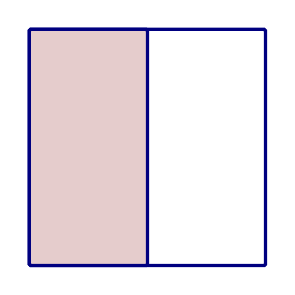
\begin{tikzpicture}[scale=3,rounded corners=.5pt]      
    \tkzDefPoint(0,0){A1} 
    \tkzDefPoint(1,0){A2}
    \tkzDefPoint(1,1){A3}
    \tkzDefPoint(0,1){A4}
    \draw[penColor,very thick] (A1)--(A2)--(A3)--(A4)--cycle;

    \tkzDefPoint(0,0){B1} 
    \tkzDefPoint(.5,0){B2}
    \tkzDefPoint(.5,1){B3}
    \tkzDefPoint(0,1){B4}
    \draw[penColor,fill=fill2,very thick] (B1)--(B2)--(B3)--(B4)--cycle;
  \end{tikzpicture}

\end{image}
There are two quantities of which we can keep track now.
\begin{itemize}
\item Call the area shaded in this step $A_1$.  Then, we have $A_1=\answer[given]{1/2}$ square units.
\end{itemize}

\paragraph{Step 2:} Shade the bottom half of the unshaded region.  

\begin{image}[1in]
  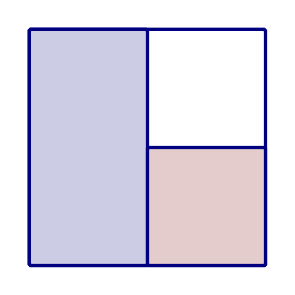
\begin{tikzpicture}[scale=3,rounded corners=.5pt]      
    \tkzDefPoint(0,0){A1} 
    \tkzDefPoint(1,0){A2}
    \tkzDefPoint(1,1){A3}
    \tkzDefPoint(0,1){A4}
    \draw[penColor,very thick] (A1)--(A2)--(A3)--(A4)--cycle;

    \tkzDefPoint(0,0){B1} 
    \tkzDefPoint(.5,0){B2}
    \tkzDefPoint(.5,1){B3}
    \tkzDefPoint(0,1){B4}
    \draw[penColor,fill=fill1,very thick] (B1)--(B2)--(B3)--(B4)--cycle;
    
    \tkzDefPoint(.5,0){C1} 
    \tkzDefPoint(1,0){C2}
    \tkzDefPoint(1,.5){C3}
    \tkzDefPoint(.5,.5){C4}
    \draw[penColor,fill=fill2,very thick] (C1)--(C2)--(C3)--(C4)--cycle;
    
  \end{tikzpicture}
\end{image}

\begin{itemize}
\item Call the new area shaded in this step $A_2$.  Then, we have $A_2=\answer[given]{1/4}$.
\item Call the total shaded area  $S_2 = A_1 + A_2$.  Then, we have $S_2=\answer[given]{3/4}$.
\end{itemize}

Visually, notice that we can find $S_2$ by noting
$$( \textrm{area shaded after Step } 2) = ( \textrm{area from Step } 1) + (\textrm{area from Step } 2)$$
and writing down the total shaded are of the square.

Analytically, we can write $S_2=A_1+A_2.$

\paragraph{Step 3:} Shade the left half of the unshaded region.  \begin{image}[1in]
  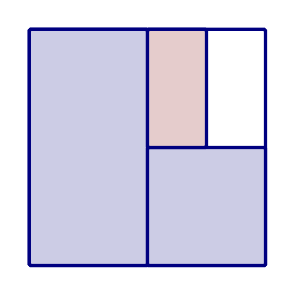
\begin{tikzpicture}[scale=3,rounded corners=.5pt]      
    \tkzDefPoint(0,0){A1} 
    \tkzDefPoint(1,0){A2}
    \tkzDefPoint(1,1){A3}
    \tkzDefPoint(0,1){A4}
    \draw[penColor,very thick] (A1)--(A2)--(A3)--(A4)--cycle;

    \tkzDefPoint(0,0){B1} 
    \tkzDefPoint(.5,0){B2}
    \tkzDefPoint(.5,1){B3}
    \tkzDefPoint(0,1){B4}
    \draw[penColor,fill=fill1,very thick] (B1)--(B2)--(B3)--(B4)--cycle;
    
    \tkzDefPoint(.5,0){C1} 
    \tkzDefPoint(1,0){C2}
    \tkzDefPoint(1,.5){C3}
    \tkzDefPoint(.5,.5){C4}
    \draw[penColor,fill=fill1,very thick] (C1)--(C2)--(C3)--(C4)--cycle;
    
    \tkzDefPoint(.5,.5){D1} 
    \tkzDefPoint(.75,.5){D2}
    \tkzDefPoint(.75,1){D3}
    \tkzDefPoint(.5,1){D4}
    \draw[penColor,fill=fill2,very thick] (D1)--(D2)--(D3)--(D4)--cycle;
    
  \end{tikzpicture}
\end{image}

\begin{itemize}
\item Call the new area shaded in this step $A_3$.  Then, we have $A_3=\answer[given]{1/8}$.
\item Call the total shaded area $S_3$.  Then, we have $S_3=\answer[given]{7/8}$.
\end{itemize}

We can think of $S_3$ visually or analytically. 

\[
S_3 = A_1 + A_2 + A_3
\]



\vspace{3mm}



Hopefully, the pattern used to shade the square is becoming clear.  We can define the new area shaded during the $n$-th step to be $A_n$, and can observe that $A_n = \left( \frac{1}{2} \right)^n$.

We can also let $S_n$ denote the total shaded area after the $n$-th step.  Analytically, we have $S_n = A_1+A_2 + \ldots A_n$, or by using summation notation, we can write $\displaystyle S_n = \sum_{k=1}^n A_k$.

Looking at the pictures drawn so far, notice that the only unshaded area after the $n$-th step is a rectangle of area $A_n$, so we can write a formula for $S_n$.   

\[
S_n = \left<\textrm{area of the whole square}\right>-A_n = 1-\left(\frac{1}{2}\right)^n
\]

We can now evaluate the limit and find that $\lim\limits_{n \to \infty} S_n =\answer[given]{1}$.

We also have another method of thinking about this limit; after we continue shading the square indefinitely, there will be no portion of it that has not been shaded.  Thus, the total shaded area should be $1$.

We would thus like to conclude that

\[
\frac{1}{2} + \left(\frac{1}{2}\right)^2+ \left(\frac{1}{2}\right)^3+ \ldots = \sum\limits_{k=1}^{\infty} \left(\frac{1}{2}\right)^n =1.
\]
\end{example}

















\section*{Infinite series}
The above scenario can be modeled using sequences.  We have $\{A_n\}_{n=1}$ whose $n$-th term is given by the explicit formula $A_n=\left(\frac{1}{2}\right)^n$, and we represent the sequence by the ordered list below.

\[
\frac{1}{2},\left(\frac{1}{2}\right)^2,\left(\frac{1}{2}\right)^3,\ldots
\]
and we can interpret the series $$\frac{1}{2} + \left(\frac{1}{2}\right)^2+ \left(\frac{1}{2}\right)^3+ \ldots$$ as the attempt to add up all of the terms in the above sequence.  In order to determine if this can be done, we found a new sequence $\{S_n\}_{n=1}$ that was created from the original sequence.  It is represented by the list below.

\[
\frac{1}{2},\frac{3}{4},\frac{7}{8},\ldots
\]

Note that the \emph{limit} of this new sequence is exactly the \emph{sum} of all of the terms in the old sequence!  Let's formalize the ideas in the last example with a definition.









\begin{definition}  \textbf{\textcolor{green!50!black}{Sequence of Partial Sums}} 


Let $\{a_n\}_{n=n_0}$ be a sequence.  Let $s_n = \sum\limits_{k=k_0}^n a_k$; the sequence $\{s_n\}_{n=k_0}$ is the called the
  \textbf{sequence of partial sums} of $\{a_n\}$.  

\begin{enumerate}
\item The series $\sum\limits_{k=k_0}^\infty a_k$ \textbf{converges} if and only if $\lim\limits_{n\to\infty} s_n$ exists.  Furthermore, if $\lim\limits_{n\to\infty} s_n =L$, we say the series $\sum\limits_{k=k_0}^\infty a_k$ converges to $L$. 
\item The series $\sum\limits_{k=k_0}^\infty a_k$ \textbf{diverges} if and only if $\lim\limits_{n\to\infty} s_n = \infty, \lim\limits_{n\to\infty} s_n = -\infty$ or $\lim\limits_{n\to\infty} s_n $ otherwise does not exist.  
\end{enumerate}
\end{definition}








The above definition really states that the symbols $\sum\limits_{k=k_0}^{\infty} a_k$ and $\lim\limits_{n \to \infty} s_n$ represent exactly the samething! It makes the content of the previous example more precise.  This is quite important since we have techniques to determine whether limits of \emph{sequences} exist.  We are now able to recast the new question ``Can I sum all of the terms in a sequence?'' into the old question ``Does the associated sequence of partial sums have a limit?".  To attack the latter, we can utilize all of our previous techniques for studying the limit of the sequence of partial sums.

\begin{remark}
Some people define the $n$-th term in the sequence of partial sums by summing the first $n$ terms in the original sequence.  With our convention, the lower index for both the original sequence and the sequence of partial sums will always be the same; that is, both sequences share a common domain.  In the case when the lower index is $k_0=1$, both conventions are equivalent.
\end{remark}









\begin{question}
  Using our new terminology, what can we say about the series $\sum\limits_{k=1}^\infty \left(\frac{1}{2}\right)^k$ from the previous example?  The series     \wordChoice{\choice[correct]{converges}\choice{diverges}}, and
      $\sum\limits_{n=1}^\infty \left(\frac{1}{2}\right)^n = \answer[given]{1}$.
  \end{question}








Now, let's see an example.

\begin{example}
Suppose that $\{a_n\}_{n=1}$ is a sequence and let $s_n = \sum\limits_{k=1}^n a_k$.  Suppose it is known that

\[
s_n = \frac{\ln(n)+5n^2}{2n^2+1}.
\]

Determine whether $\sum\limits_{k=1}^{\infty} a_k$ converges or diverges.  If it converges, give its value.

\begin{explanation}
The symbols $\sum\limits_{k=1}^{\infty} a_k$ and $\lim\limits_{n \to \infty} s_n$ are equivalent; in order to determine whether $\sum\limits_{k=1}^{\infty} a_k$ converges or diverges, we need to analyze $\lim\limits_{n \to \infty} s_n$.  

\begin{itemize}
\item The dominant term in the numerator is \wordChoice{\choice{$\ln(n)$}\choice[correct]{$5n^2$}}.
\item The dominant term in the denominator is \wordChoice{\choice[correct]{$2n^2$}\choice[correct]{$1$}}.
\end{itemize}
We can conclude that 

\[ \lim\limits_{n \to \infty} s_n = \lim\limits_{n \to \infty} \frac{\ln(n)+5n^2}{2n^2+1} =  \lim\limits_{n \to \infty} \frac{5n^2}{2n^2} = \answer[given]{\frac{5}{2}}\]

Hence, $\sum\limits_{k=1}^{\infty} a_k$ converges since  $\lim\limits_{n \to \infty} s_n$ exists, and since  $\lim\limits_{n \to \infty} s_n=\frac{5}{2}$, we have that $\sum\limits_{k=1}^{\infty} a_k$ converges to $\frac{5}{2}$.
\end{explanation}

\end{example}














\section*{Properties of sums}

We finish this section by giving some properties of series.

\begin{theorem}[Sums and Constant Multiples of Convergent Series]
  Let  $\sum\limits_{k=k_0}^\infty a_k$ and  $\sum\limits_{k=k_0}^\infty b_k$ be \emph{convergent} series and suppose that $
  \sum\limits_{k=k_0}^\infty a_k = A$ and $\sum\limits_{k=k_0}^\infty b_k =B.$
 
 \begin{enumerate}
\item Constant Multiple Rule 

For any constant $c$, \[\sum\limits_{k=k_0}^\infty c\cdot a_k =
  c\cdot\sum\limits_{k=k_0}^\infty a_k = c\cdot A.\]\index{series!Constant Multiple
    Rule}
\item Sum/Difference Rule 

\[\sum\limits_{k=k_0}^\infty \big(a_k\pm b_k\big) =
  \sum\limits_{k=k_0}^\infty a_k \pm \sum\limits_{k=k_0}^\infty b_k = A \pm B.\]
  \index{series!properties}\index{series!Sum/Difference Rule}
\end{enumerate} 
\end{theorem}


Notice, of course, that we're working with convergent series in this 
theorem.  Adding divergent series is trickier, but there is something we can say about the attempt to add a convergent series and a divergent series.

\begin{theorem}
 Suppose $\sum\limits_{k=k_0}^\infty a_k$ converges and  $\sum\limits_{k=k_0}^\infty b_k$ diverges.  Then, $\sum\limits_{k=k_0}^{\infty} \big(a_k+b_k\big)$ diverges.
\end{theorem}

To understand why this theorem holds, note that if $\sum\limits_{k=k_0}^\infty \big(a_k+b_k\big)$ would converge, by the last theorem, we would know that the difference

\[\sum\limits_{k=k_0}^\infty \big(a_k+b_k\big) -\sum\limits_{k=k_0}^\infty a_k\]
converges since both series above are convergent.  Furthermore, the previous theorem also guarantees that

\[\sum\limits_{k=k_0}^\infty \big(a_k+b_k\big) -\sum\limits_{k=k_0}^\infty a_k = \sum\limits_{k=k_0}^\infty \big(a_k+b_k -a_k\big),\]

but this is precisely $\sum\limits_{k=k_0}^{\infty} b_k$, which diverges by assumption.  This is a contradiction, so  $\sum\limits_{k=k_0}^\infty \big(a_k+b_k\big)$ must diverge.


\begin{theorem}[Convergence of Tails]
  Let $\{a_n\}_{n=n_0}$ be a sequence and $n_1 \geq n_0$ be an integer.  Then, $\sum\limits_{k=n_0}^{\infty} a_k$ and $\sum\limits_{k=n_1}^{\infty} a_k$ either both converge or both diverge.
\end{theorem}

Essentially, this theorem ensures that it does not matter where we \emph{start} summing the terms of a sequence.  Since we have infinitely many terms to try to add together, the sum of the first finitely many will not affect \emph{if} this addition is possible.

\begin{remark}
If $n_1>n_0$, the series $\sum\limits_{k=n_1}^{\infty} a_k$ is often called a \emph{tail} of the series $\sum\limits_{k=n_0}^{\infty} a_k$.
\end{remark}

We now finish the section with an example that ties many ideas together.


%%%%%%%%%%%
\begin{example}
Suppose that $\{a_n\}_{n=1}$ is a sequence and define its sequence of partial sums $\{s_n\}_{n=1}$ by the usual rule $s_n = \sum\limits_{k=1}^n a_k$.  Suppose it is known that

\[
s_n = \frac{8n^2}{n^4-9}.
\]

\begin{question}
What is $a_1+a_2+a_3$?  \wordChoice{\choice[correct]{$1$}\choice{$\frac{18}{7}$}\choice{It is not defined.}}

\begin{explanation}
Note that we are given an explicit formula for the term $s_n$.  By definition, we have $s_3 = a_1+a_2+a_3$, so all we have to do to find $a_1+a_2+a_3$ is to evaluate the formula for $s_n$ when $n=3$.

\[
a_1+a_2+a_3 = s_3 = \frac{8(3)^2}{(3)^4-9} = 1
\]

\end{explanation}
\end{question}

\begin{question}
What is $a_2+a_3$?

\begin{explanation}
Note that $s_3 = a_1+a_2+a_3$ and $s_1 = a_1$.  Thus, 

\[s_3 -s_1 = \left(\cancel{a_1}+ a_2+a_3\right) -\cancel{a_1} = a_2+a_3\]

Using the formula for $s_n$ gives $s_3 = \answer[given]{1}$ and $s_1=\answer[given]{-1}$, so $a_2+a_3 =  \answer[given]{2}$.
\end{explanation}
\end{question}

\begin{question}
Determine whether $\sum\limits_{k=1}^{\infty} a_k$ converges or diverges.  If it converges, what is its value?

\begin{explanation}
We can determine whether $\sum\limits_{k=1}^{\infty} a_k$ converges or diverges by analyzing $\lim\limits_{n \to \infty} s_n = \lim\limits_{n \to \infty} \frac{8n^2}{n^4-9}$.  Since this limit is zero, we know that $\sum\limits_{k=1}^{\infty} a_k$ converges to $0$.
\end{explanation}
\end{question}

\begin{question}
Determine whether $\sum\limits_{k=4}^{\infty} a_k$ converges or diverges.  If it converges, can you find its value?

\begin{explanation}
Since $\sum\limits_{k=1}^{\infty} a_k$ converges, changing the lower index to $k=4$ \wordChoice{\choice{will}\choice[correct]{will not}}  affect whether the series converges.  Since we found that $\sum\limits_{k=1}^{\infty} a_k$ converges, so too will $\sum\limits_{k=4}^{\infty} a_k$.  However, since $k=4$ is our lower index here, it \wordChoice{\choice[correct]{will}\choice{will not}} potentially affect the value of the series.

Let's write out the series and make a few observations.

\begin{image}
  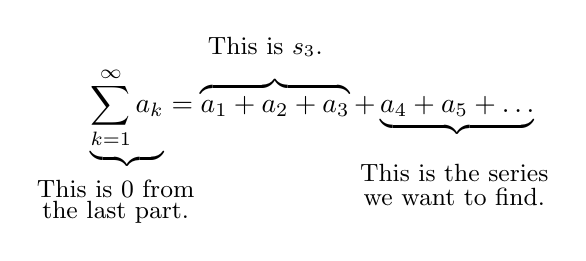
\begin{tikzpicture}
        \node at (0,0) {
          $\underbrace{\sum_{k=1}^{\infty} a_k}=\overbrace{a_1+a_2+a_3}+ \underbrace{a_4+a_5 + \ldots}$};
        \node at (1.8,-.7) {\small{This is the series}};
        \node at (1.8,-1) {\small{we want to find.}};
        
        \node at (-2.5,-.9) {\small{This is $0$ from }};
        \node at (-2.5,-1.2) {\small{the last part.}};    
        
        \node at (-.6,.9) {\small{This is $s_3$. }};
        
      \end{tikzpicture}
  \end{image}
  
 Putting this together, we have:
 
 \[
 0 = s_3 + \sum\limits_{k=4}^{\infty} a_k,
 \] 
 and we find that $ \sum\limits_{k=4}^{\infty} a_k = -1$. 

We can determine whether $\sum\limits_{k=1}^{\infty} a_k$ converges or diverges by analyzing $\lim\limits_{n \to \infty} s_n = \lim\limits_{n \to \infty} \frac{8n^2}{n^4-9}$.  Since this limit is zero, we know that $\sum\limits_{k=1}^{\infty} a_k$ converges to $0$.
\end{explanation}
\end{question}

\end{example}













\begin{center}
\textbf{\textcolor{green!50!black}{ooooo-=-=-=-ooOoo-=-=-=-ooooo}} \\

more examples can be found by following this link\\ \link[More Examples of Sums of Sequences]{https://ximera.osu.edu/csccmathematics/precalculus1/precalculus1/sumsOfSequences/examples/exampleList}

\end{center}





\end{document}
